\section{Data storage and management system}

\subsection{The \pd Data Characteristics}
The characteristics of the \pd data determine the scale and possible design
options for its computing infrastructure.
These characteristics are in a large part defined by a few fundamental
properties of the \pd Liquid Argon TPC:
\begin{itemize}
\item High spatial granularity of readout (e.g. the pitch of the electrode pattern etc), and the resulting high channel count
\item High digitization frequency (which is essential to ensure a precise position measurement along the drift direction)
\item Relatively slow drift velocity of electrons in Liquid Argon, which  leads to a substantial readout window (of the order of milliseconds) required to collect
all of the ionization in the Liquid Argon volume due the event of interest. 
\end{itemize}

\noindent Combination of these factors leads to a considerable amount of data per
event and depending on
the chosen run plan (i.e. trigger rate and total required statistics) may result in considerable requirements
regarding the bandwidth and storage. These can be illustrated as follows.

The \textit{``\pd/SP Data Scenarios''} spreadsheet\,\cite{data_spreadsheet}
(DUNE DocDB 1086)
describes three possible running conditions and estimates for their
resulting data volumes and rates and interpretations in terms of
network and disk bandwidth.  It also includes estimates for non-beam
trigger for acquiring additional cosmic-$\mu$ data.  Some highlights
of these estimates for the mid-range (so-called ``Goldilocks'')
scenario are in Table~\ref{tab:goldi}. The lossless compression factor cited
in the table is based on the assumption that noise level are under control
and of the same order or better as in $\mu$BooNE.

\begin{table}[htbp]
  \centering
  \begin{tabular}[h]{l|r}
\hline
    Trigger rate & \SI{10}{\Hz} \\
    Spill duration & \SI{4.8}{\second} \\
    SPS Cycle & \SI{16.8}{\second} \\
    Readout time window & \SI{5}{\milli\second} \\
    \# of APAs to be read out & 3 \\
    \hline
    Single readout size (per trigger) & \SI{115}{\mega\byte} \\
    Compression factor & 5 \\
    Instantaneous data rate & \SI{230}{\mega\byte\per\second} \\
    Average data rate & \SI{66}{\mega\byte\per\second} \\
    \hline
    3-Day buffer depth & \SI{17}{\tera\byte} \\
    \hline
  \end{tabular}
  \caption{Parameters defining data rate and volume in the ``Goldilocks'' scenario v5\,\cite{data_spreadsheet}.}
  \label{tab:goldi}
\end{table}

Based on preliminary plan for calibrations which involves measuring a few types of cosmic $\mu$ tracks
(e.g. at different angles, stopped vs not stopped etc),
the current assumption is that for every beam trigger one non-beam
trigger be acquired out-of-spill. 
This assumption represents a doubling of the data rates and volumes presented in Table~\ref{tab:goldi}.
The instant and average rates are those for when the beam is spilling or if the rate is amortized over the
entire beam cycle. 

The current run plan calls for about 5\,M beam events to be collected in the first run of \pd. Triggers (such as PID) will be
actuated using beam instrumentation which is being developed at the time of writing. Its efficiency will certainly be less
than 100\,\% and for estimation purposes is assumed to be 50\,\%. This leads to the requested total statistics of 10\,M
events. Combined with readout size quoted in Table\,\ref{tab:goldi} it results in the anticipated volume of raw data of
about 0.5\,PB to be taken during the SPS run. To account for commissioning of the detector this estimate should be roughly doubled,
resulting in estimated 1\,PB of raw data.


%%%%%%%%%%%%%%% Tom's stuff
\subsection{Interface of the DAQ to the online storage}
% -mxp- commenting out Tom's intro... To save page count
%Just like in many other experiments, the \pd data rate depends on the number of
%triggers needed in order to meet the test and measurement goals, and
%the operating schedule.

%The requirements that the data handling and processing system has to meet are
%determined most  by the desired data rate and, to a lesser extent, the total data volume.
%On the other hand, available funding and personnel place
%constraints on the size and functionality of the online data handling
%and processing system. This makes it necessary to carefully design
%the run program and optimize the system for maximum efficiency and
%performance.


Table\,\ref{tab:goldi} contains the nominal trigger rate of 10\,Hz for
the mid-range scenario. It may be necessary to provide the capability
to run at  an instantaneous trigger rate of up to 100\,Hz in order to
allow for commissioning and schedule delays. For that reason,
scalability of the DAQ, the online buffer and the prompt processing system
\ref{sec:prompt_processing} is an important design requirement.
% the DAQ and online processing system is designed to handle. 
%Up to six APA modules are to be read out on
%each trigger.  The data are assumed to be compressed in the RCE's,
%with a lossless compression ratio of 5.
 Data are assumed to be
collected based on prompt trigger signals generated by the beamline
instrumentation in order to purify samples of desired particles.

The readout of the photon detector channels and the beam
instrumentation is assumed to be a relatively minor addition to the
total data rate and are not anticipated to drive the design of the
data handling and processing system, although adequate resources must
be provisioned in order to acquire and store the data from these
systems.

The network speed of all computers in the data acquisition
chain is anticipated to be 10\,Gbits/sec.  Computers running near-line
processing of subsets of the data, which are generally CPU-bound, may
be connected with 1\,GBit/sec links.  The software framework for
interfacing with the electronics, building events, writing data files,
and providing an interface to online monitoring of data as it is
acquired is {\it artdaq}~\cite{artdaq}.

Assuming that each RCE reads out 128 channels of the TPC, 120 RCE's
will need to be active.  Twelve computers running BoardReader
processes will read out ten RCE's each.  These computers should be
provisioned with at least 8 cores and 16 GBytes of RAM each, along
with a 10\,Gbit/sec network connection.  The BoardReader processes will
transmit data to a set of computers running EventBuilder processes.
Sixteen EventBuilder computers, each with 8 cores and 16\,GB of RAM
and a 10\,Gbit/sec NIC will provide the CPU and networking needed to
build events, perform basic online monitoring, and send the data to
disk storage.  The EventBuilders assemble data fragments sent by the
BoardReaders into self-consistent events consisting of readout data
from each contributing RCE, SSP, and beam instrumentation information
for the same time period.  They will also perform basic data integrity
checks, ensuring that all data that are expected for an event have
arrived and have not been corrupted, before writing records out.

The disk storage layer will consist of 350\,TB of high-speed
disks, which may be connected directly or network-attached.  As of this writing, the filesystem and
interface software layer is not yet defined, but may be one of the
following --
% an instance of EOS~\cite{eos},
a XRootD cluster~\cite{xrootd}, a SAN installation, or
simply disks locally attached to the EventBuilder computers.  A
alternative to this design that allows for more flexibility but at a
cost of network latency and CPU, is to add a layer of Aggregator CPU
processes between the EventBuilders and the disk writing.  These
processes may be needed if the events are to be sorted, analyzed,
reformatted, or otherwise handled before writing out.  In order to
maximize throughput and minimize cost, the number of steps in the data
handling system is to be minimized.

After the data are written to disk by {\it artdaq}, the data handling
system creates metadata files, runs near-line monitoring jobs, and
transfers the data from EHN1 to the CERN Computing Centre, as
described in DUNE DocDB~1212~\cite{docdb1212}. According to the current plan,
the ``F-FTS'' software developed and maintained at FNAL will be the centerpiece
of managing the data flow at this level.


\subsection{Raw Data Flow in \pd}
\label{sec:raw_concept}
%%%%%%%%%%%%%%%%%%%%%%%%
\begin{figure}[tbh]
\centering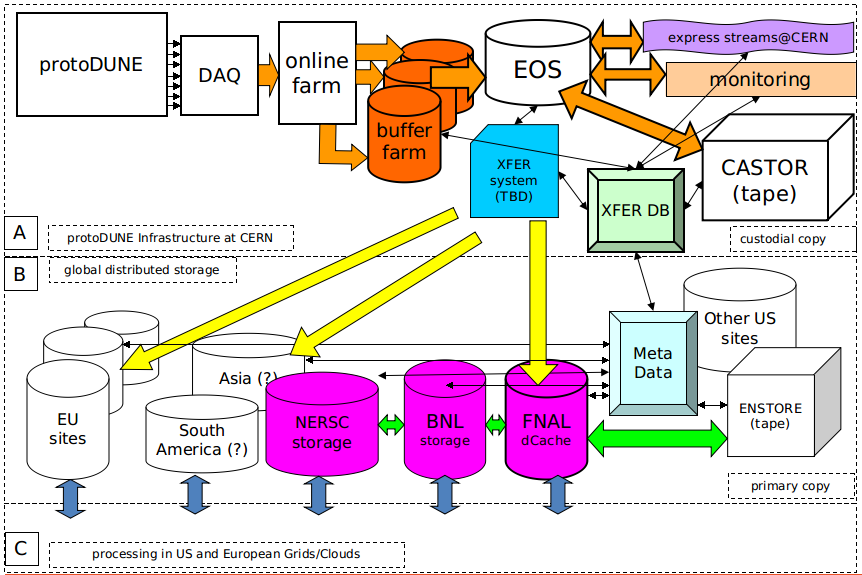
\includegraphics[width=\linewidth]{protoDUNE_raw_data_concept.png}
\caption{\label{fig:raw_concept}Conceptual diagram of the flow of raw data in \pd}
\end{figure}
%%%%%%%%%%%%%%%%%%%%%%%%

\noindent
Conceptual diagram of the raw data flow in \pd is presented in Fig.\ref{fig:raw_concept}. It shows the general logic
of data flow, and does not include specific assumptions about what system will be used to actually move the data.
It also reflects the central role of CERN EOS in the \pd raw data management scheme. This is motivated by the experience
and architecture of the LHC experiments.

EOS serves as the staging area from which the data gets committed to CASTOR
and from which it is transmitted to a number of endpoints including principal data centers such as FNAL and others.
It is also used to provide input to QA and other express processing streams at CERN (sec.\,\ref{sec:prompt_processing}).
%This scheme assumes that there is no conceptual difference between NP02 and NP04 in terms of the general pattern of data flow.

Data centers at BNL and NERSC are placed in this diagram for illustration purposes. Any other institution possessing adequate
resources can participate in this data distriburtion scheme if desired. According to the design presented in DUNE DocDB~1212~\cite{docdb1212}
this part of the data transmission process is also handled by an instance of F-FTS.


